\documentclass{article}
\usepackage{setspace}
\usepackage{amsmath}
\usepackage{amssymb}
\usepackage{amsthm}
\usepackage{graphicx} 
\usepackage{float} 
\usepackage{fancyhdr}                                
\usepackage{lastpage}        
\usepackage{siunitx} 
\usepackage{textcomp}                               
\usepackage{layout}   
\usepackage{subfigure} 
\pagestyle{fancy}  
\lhead{ZHANG HUAKANG}
\chead{Assignment 1} 
\rhead{DB92760} 
\title{Assignment 1 of CISC 3018}
\author{ZHANG HUAKANG}
\begin{document}
    \maketitle
    \section{}
        \subsection*{C/S service model}
        $$d_{CS}=max\{\frac{NF}{u_s},\frac{F}{{min}_i(d_i)}\}$$
        \subsection*{P2P model}
        $$d_{P2P}=max\{\frac{F}{u_s},\frac{F}{{min}_i(d_i)},\frac{NF}{u_s+\sum u_i}\}$$
        \subsection{}
            \subsection*{$N=5$}
                \begin{equation*}
                    \begin{split}
                        d_{CS}=&max\{\frac{NF}{u_s},\frac{F}{{min}_i(d_i)}\}\\
                            =&max\{\frac{5\times 20MBits}{40MHz},\frac{20MBits}{10MHz}\}\\
                            =&{\frac{5}{2}}{ Bits/Hz}
                    \end{split}
                \end{equation*}
            \subsection*{$N=10$}
                \begin{equation*}
                    \begin{split}
                        d_{CS}=&max\{\frac{NF}{u_s},\frac{F}{{min}_i(d_i)}\}\\
                            =&max\{\frac{10\times 20MBits}{40MHz},\frac{20MBits}{10MHz}\}\\
                            =&{5}{ Bits/Hz}
                    \end{split}
                \end{equation*}
            \subsection*{$N=20$}
                \begin{equation*}
                    \begin{split}
                        d_{CS}=&max\{\frac{NF}{u_s},\frac{F}{{min}_i(d_i)}\}\\
                            =&max\{\frac{20\times 20MBits}{40MHz},\frac{20MBits}{10MHz}\}\\
                            =&{10}{ Bits/Hz}
                    \end{split}
                \end{equation*}
            \subsection*{$N=40$}
                \begin{equation*}
                    \begin{split}
                        d_{CS}=&max\{\frac{NF}{u_s},\frac{F}{{min}_i(d_i)}\}\\
                            =&max\{\frac{40\times 20MBits}{40MHz},\frac{20MBits}{10MHz}\}\\
                            =&{20}{ Bits/Hz}
                    \end{split}
                \end{equation*}
            \subsection*{$N=60$}
                \begin{equation*}
                    \begin{split}
                        d_{CS}=&max\{\frac{NF}{u_s},\frac{F}{{min}_i(d_i)}\}\\
                            =&max\{\frac{60\times 20MBits}{40MHz},\frac{20MBits}{10MHz}\}\\
                            =&{30}{ Bits/Hz}
                    \end{split}
                \end{equation*}
        \subsection{}
            \subsubsection*{$N=5$}
                \begin{equation*}
                    \begin{split}
                        d_{P2P}=&max\{\frac{F}{u_s},\frac{F}{{min}_i(d_i)},\frac{NF}{u_s+\sum u_i}\}\\
                            =&max\{\frac{20MBits}{40MHz},\frac{20MBits}{10MHz},\frac{5\times 20MBits }{40MHz+5\times 5MHz}\}\\
                            =&\frac{20}{13}Bits/Hz
                    \end{split}
                \end{equation*}
            \subsubsection*{$N=10$}
                \begin{equation*}
                    \begin{split}
                        d_{P2P}=&max\{\frac{F}{u_s},\frac{F}{{min}_i(d_i)},\frac{NF}{u_s+\sum u_i}\}\\
                            =&max\{\frac{20MBits}{40MHz},\frac{20MBits}{10MHz},\frac{10\times 20MBits }{40MHz+10\times 5MHz}\}\\
                            =&\frac{20}{9}Bits/Hz
                    \end{split}
                \end{equation*}
            \subsubsection*{$N=20$}
                \begin{equation*}
                    \begin{split}
                        d_{P2P}=&max\{\frac{F}{u_s},\frac{F}{{min}_i(d_i)},\frac{NF}{u_s+\sum u_i}\}\\
                            =&max\{\frac{20MBits}{40MHz},\frac{20MBits}{10MHz},\frac{20\times 20MBits }{40MHz+20\times 5MHz}\}\\
                            =&\frac{20}{7}Bits/Hz
                    \end{split}
                \end{equation*}
            \subsubsection*{$N=40$}
                \begin{equation*}
                    \begin{split}
                        d_{P2P}=&max\{\frac{F}{u_s},\frac{F}{{min}_i(d_i)},\frac{NF}{u_s+\sum u_i}\}\\
                            =&max\{\frac{20MBits}{40MHz},\frac{20MBits}{10MHz},\frac{40\times 20MBits }{40MHz+40\times 5MHz}\}\\
                            =&\frac{10}{3}Bits/Hz
                    \end{split}
                \end{equation*}
            \subsubsection*{$N=60$}
                \begin{equation*}
                    \begin{split}
                        d_{P2P}=&max\{\frac{F}{u_s},\frac{F}{{min}_i(d_i)},\frac{NF}{u_s+\sum u_i}\}\\
                            =&max\{\frac{20MBits}{40MHz},\frac{20MBits}{10MHz},\frac{60\times 20MBits }{40MHz+60\times 5MHz}\}\\
                            =&\frac{60}{17}Bits/Hz
                    \end{split}
                \end{equation*}
        \subsection{}
            \begin{equation*}
                \begin{split}
                    F=&20MBits,\\
                    u_s=&40MHz,\\
                    min_i(d_i)=&10MHz,\\
                    u_i=&5Mhz\\
                \end{split}
            \end{equation*}
            \begin{equation*}
                \begin{split}
                    d_{CS}(N;F,u_s,d_i,u_i)=&max\{\frac{NF}{u_s},\frac{F}{{min}_i(d_i)}\}\\
                        =&max\{\frac{N\times 20MBits}{40MHz},\frac{20MBits}{10MHz}\}\\
                        =&max\{\frac{N}{2},\frac{1}{2}\}Bits/Hz\\
                        =&\frac{N}{2}Bits/Hz
                \end{split}
            \end{equation*}
            \begin{equation*}
                \begin{split}
                    d_{P2P}(N;F,u_s,d_i,u_i)=&max\{\frac{F}{u_s},\frac{F}{{min}_i(d_i)},\frac{NF}{u_s+\sum u_i}\}\\
                        =&max\{\frac{20MBits}{40MHz},\frac{20MBits}{10MHz},\frac{N\times20MBits}{40MHz+N\times 5MHz}\}\\
                        =&max\{\frac{1}{2},\frac{1}{2},\frac{4N}{8+N}\}Bits/Hz\\
                \end{split}
            \end{equation*}
            We can get:
            $$\frac{4N}{8+N}-\frac{1}{2}=\frac{3N-8}{16+2n}.$$
            When $3N-8>0$, i.e. $N\geq 3>\frac{8}{3}$
                $$d_{P2P}(N;F,u_s,d_i,u_i)=\frac{4N}{8+N}Bits/Hz$$
            and when $3N-8\leq 0$, i.e. $0\leq N\leq 2 <\frac{8}{3}$
                $$d_{P2P}(N;F,u_s,d_i,u_i)=\frac{1}{2}Bits/Hz$$
            When $N=5,10,20,40,60$,
                \begin{equation*}
                    \begin{split}
                        \Delta_{CS,P2P}(5)=&\frac{25}{26}Bits/Hz\\
                        \Delta_{CS,P2P}(10)=&\frac{25}{9}Bits/Hz\\
                        \Delta_{CS,P2P}(20)=&\frac{50}{7}Bits/Hz\\
                        \Delta_{CS,P2P}(40)=&\frac{50}{3}Bits/Hz\\
                        \Delta_{CS,P2P}(60)=&\frac{450}{17}Bits/Hz
                    \end{split}
                \end{equation*}
                \paragraph{
                    We can know that as $N$ becomes larger, the difference between the two will become larger and larger, and the advantages of P2P will become more and more obvious 
                }

        \subsection{}
            \paragraph{
                \begin{equation*}
                    \begin{split}
                        \lim_{N\rightarrow \infty}d_{CS}(N;F,u_s,d_i,u_i)=&\lim_{N\rightarrow \infty}\frac{N}{2}Bits/Hz\\
                            =&\infty\\
                        \lim_{N\rightarrow \infty}d_{P2P}(N;F,u_s,d_i,u_i)=&\lim_{N\rightarrow \infty}\frac{4N}{8+N}Bits/Hz\\
                            =&\infty
                    \end{split}
                \end{equation*}
                \begin{equation*}
                    \begin{split}
                        \lim_{N\rightarrow \infty}\frac{d_{P2P}(N;F,u_s,d_i,u_i)}{d_{CS}(N;F,u_s,d_i,u_i)}=&\lim_{N\rightarrow \infty}\frac{\frac{4N}{8+N}}{\frac{N}{2}}\\
                            =&\lim_{N\rightarrow \infty}\frac{8}{8+N}\\
                            =&0
                    \end{split}
                \end{equation*}
                But,
                when $N>3$,
                \begin{equation*}
                    \begin{split}
                        \Delta_{CS,P2P}(N)=&(\frac{N}{2}-\frac{4N}{8+N})Bits/Hz\\
                            =&\frac{N^2}{16+2N}Bits/Hz\\
                    \end{split}
                \end{equation*}
                \begin{figure}[H]
                    \centering
                    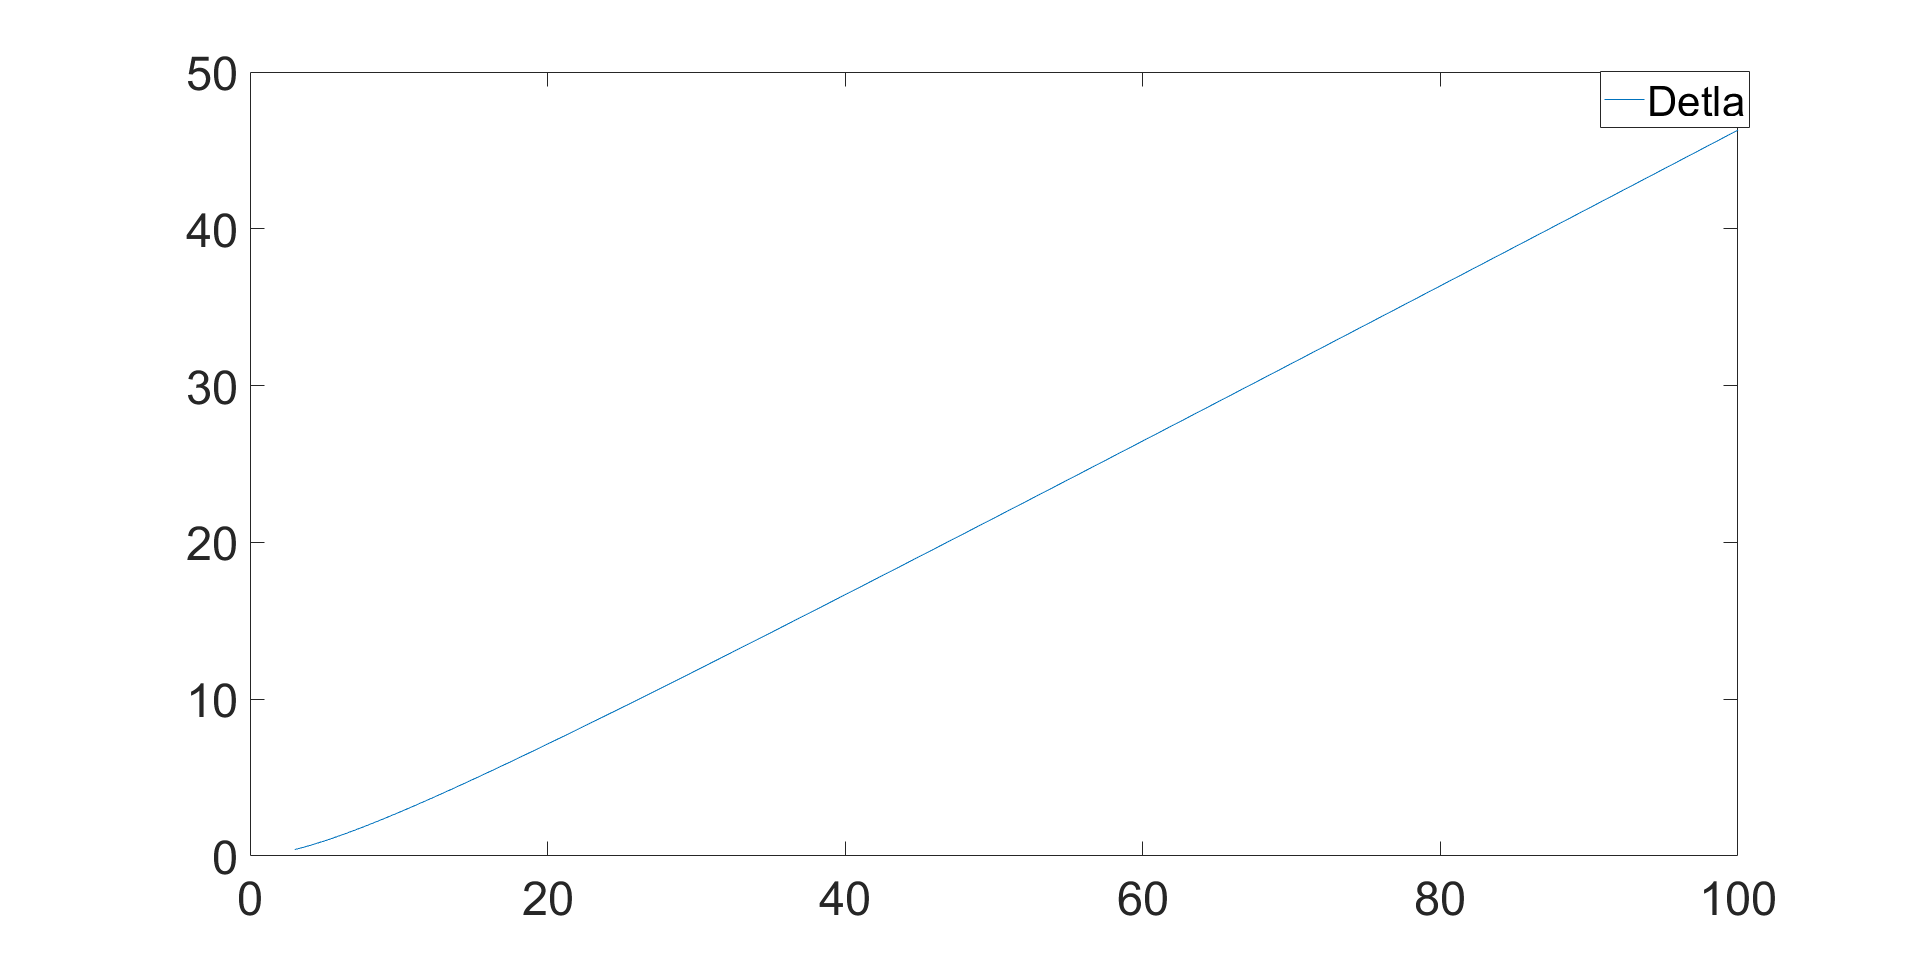
\includegraphics[width=01\textwidth]{img/Assignment1-1.png}
                \end{figure}
                We can know that as $N$ is infty, both of them will need infty time to finish the distribution, but the difference between the two will become larger and larger, and the advantages of P2P will become more and more obvious 
            }
            
\end{document}